\chapter{Compilation}
The following chapter will present the design for the reversible heap manager and the translation schemes used in the process of translating \rooplpp to the reversible low-level machine language \textsc{PISA}.

\section{Dynamic Memory Management}
Native support of complex data structures is not a trivial matter to implement in a reversible computing environment. Variable-sized records and frames need to be stored efficiently in a structured heap, while avoiding garbage build-up to maintain reversibility. A reversible heap manager layout has been proposed for a simplified version of the reversible functional language \textsc{RFun} and later expanded to allow references to avoid deep copying values~\cite{ha:heap, ty:rfun, tm:refcounting}.\\

The following section presents a discussion of various heap manager layouts along with their advantages and disadvantages in terms of implementation difficulty, garbage build-up and the OOP domain. 

\subsection{Heap manager layout}
Heap managers can be implemented in numerous ways. Different layouts yield advantages when allocating memory, finding a free block or when collecting garbage. As our goal is to construct a garbage-free heap manager, our finalized design should emphasize and reflect this objective in particular. Furthermore, we should attempt to allocate and deallocate memory as efficiently as possible, as merging and splitting of blocks is a non-trivial problem in a reversible setting.\\

% Something about OS assumptions
For the sake of simplicity, we will not consider the the issue of retrieving memory pages reversibly. A reversible operating system is a long-term dream of the reversible programmer and as reversible programming language designers, we assume that \rooplpp will be running in a  environment, in which the operating system will be supplying memory pages and their mappings. As such, the following heap memory designs reflect this preliminary assumption, that we always can query the operating system for more memory. \\

% Something about what other compilers do
Historically, most object-oriented programming languages utilize a dynamic memory manager during program execution. In older, lower-level languages such as \textsc{C}, memory allocation had to be stated explicitly and with the requested size through the \texttt{malloc} statement and deallocated using the \texttt{free} statement. Modern languages, such as \textsc{C\texttt{++}}, \textsc{Java} and \textsc{Python}, \textit{automagically} allocates and frees space for objects and variable-sized arrays by utilizing their dynamic memory manager to dispatch \texttt{malloc}- and \texttt{free}-like operations to the operating system and managing the obtained memory blocks in private heap(s)~\cite{wh:cpp_memory, bv:jvm, py:memory}. The heap layout of these managers vary from language to language and compiler to compiler.\\

% Reversible Heaps
Previous work on reversible heap manipulation has been done for reversible functional languages in~\cite{ha:heap, jsk:translation, tm:garbage}.\\


% TODO: Something about Cons/Nil heap
\texttt{TODO: Something about Cons/Nil heap from~\cite{ha:heap}}\\

% TODO: Modifications to said 
\texttt{TODO: Something about ref count extension~\cite{tm:refcounting}}

\subsubsection{Memory Pools}
A simple layout for a heap manager would allocate memory using fixed-size blocks regardless of the actual size of the record, which is known as memory pooling~\cite{bk:memorypool}. The advantage of a heap layout following this approach would lie in the simplicity of its implementation, as simple a linked list of identical-sized free cells would need to be maintained. If we assume a our fixed-sized blocks are of size $n$ machine words, the following \texttt{get\_free} subroutine allocates and deallocates memory cells for a record of size $m$.
\begin{lstlisting}[mathescape=true, frame=single, caption={Allocating and deallocating records of size $m$ using block of a fixed size $n$. Code modified from~\cite{ha:heap}}, captionpos=b, language=janus]
if ($r_{flp}$ == 0) 
then
	XOR $r_{cell}$ $r_{hp}$
	ADDI $r_{hp}$ $m + (m \% n)$ 
else
	EXCH $r_{cell}$ $r_{flp}$
	SWAP $r_{cell}$ $r_{flp}$
fi ($r_{flp}$ == 0) && ($r_{cell}$ == $r_{hp}$ - $m + (m \% n)$)
\end{lstlisting}
A huge disadvantage to using fixed-sized memory blocks is the fragmentation that occurs when freeing blocks. When freeing a number of blocks in the middle of a section of allocated blocks, fragmentation occurs, which becomes a problem if we need to allocate space for a large record but only have small sections of fixed-blocks available, scattered throughout the heap. A garbage collector could solve this issue, but is a non-trivial matter to implement.\\

\texttt{TODO: Graphics}


\subsubsection{Buddy Memory}
In this approach we have all blocks be variable-size of the power-of-two. Having different block sizes and methods for splitting a larger block into smaller ones reduces fragmentation. In terms of implementation, reversible splitting and merging might be possible as we're always doubling the size when merging and halving when splitting, thus making the operations logically inverse of each other~\cite{dk:buddyalloc}.\\

Assuming we have access to an array of pointers $flps[]$, pointing to the beginning of a free list, index at its power-of-two, we could allocate and deallocate a record of size $n$ in the following manner
\begin{lstlisting}[mathescape=true, frame=single, caption={Allocating and deallocating records of size $n$ using Buddy Memory}, captionpos=b, language=janus]
powerOfTwo = 2
while (powerOfTwo < n)
	powerOfTwo = powerOfTwo * 2
	
if (flps[powerOfTwo] == 0) 
then
	XOR $r_{cell}^{powerOfTwo}$ $r_{hp}^{powerOfTwo}$
	ADDI $r_{hp}^{powerOfTwo}$ powerOfTwo 
else
	EXCH  $r_{cell}^{powerOfTwo}$ flps[powerOfTwo]
	SWAP $r_{cell}^{powerOfTwo}$ flps[powerOfTwo]
fi (flps[powerOfTwo] == 0) && ($r_{cell}^{powerOfTwo}$== $r_{hp}^{powerOfTwo}$ - powerOfTwo)
\end{lstlisting}

\texttt{TODO: Should growing/shrinking be handled here?}\\

\texttt{TODO: Graphics}

\subsubsection{One heap per record type}
Another layout approach would be maintaining one heap per record type in the program. During compilation, classes would be analysed and a heap for each class would be created. The advantage of this approach would be less garbage generation, as each allocation is tailored as closely as possible to the size of the record obtained from a static analysis during compilation. The obvious disadvantage is the amount of book-keeping and workload associated with growing and shrinking a heap and its neighbours.

\texttt{Algorithm: Determine heap for record type, call get\_free on found heap}\\

\texttt{TODO: Graphics}

\subsubsection{Shared heap, record type-specific free lists}
A combination of the previous layouts would consist of a single heap, but record-specific free lists. This way, we ensure minimal fragmentation when allocating and freeing as the different free lists ensures that allocation of an object wastes as little memory as possible. By only keeping one heap, we eliminate the growth/shrinking issues of the multiple heap layout. There is, however, still a considerable amount of book-keeping involved in maintaining multiple free-lists. The bigger the number of unique classes defined in a program, the more free-lists we need to maintain during execution. If the free-lists are not allowed to point at the same free block (which they intuitively shouldn't in order to ensure reversibility), programs with many classes, say one hundred, could potentially fill up the heap with one hundred free lists, but only ever allocate objects for one of the classes, thus wasting a lot of memory on unused free lists. This scenario could potentially be avoided with compiler optimizations.\\

\texttt{Algorithm: Find block size for record type-specific free list, call get\_free on shared heap}\\

\texttt{TODO: Graphics}

\subsubsection{One heap per power-of-two}
A different approach as to having one heap per record type, would be having one heap per power-of-two until some arbitrary size. Using this approach, records would be stored in the heap which has a block size of a power-of-two closes matching to the record's size. This layout is a distinction from the "one heap per record type" as it still retains the size-optimized storing idiom but allows the heaps to contain records of mixed types. For programs with a large amount of small, simple classes needed to model some system, where each class is roughly the same size, the amount of heaps constructed would be substantially smaller than using one heap per record type, as many records will fit within the same heap. Implementation wise, the number of heaps can be determined at compile time. Furthermore, to ensure we do not end up with heaps of very large memory blocks, an arbitrary power-of-two size limit could be set at, say, 1 kb . If any record exceeds said limit, it could be split into $\sqrt{n}$ size chunks and stored in their respective heaps.\\
This approach does, however, also suffer from large amount of book-keeping and fiddling when shrinking and growing adjacent heaps.\\

\texttt{Algorithm: Similar to buddy memory?}\\

\texttt{TODO: Graphics}

\begin{figure}[H]
  \centering
  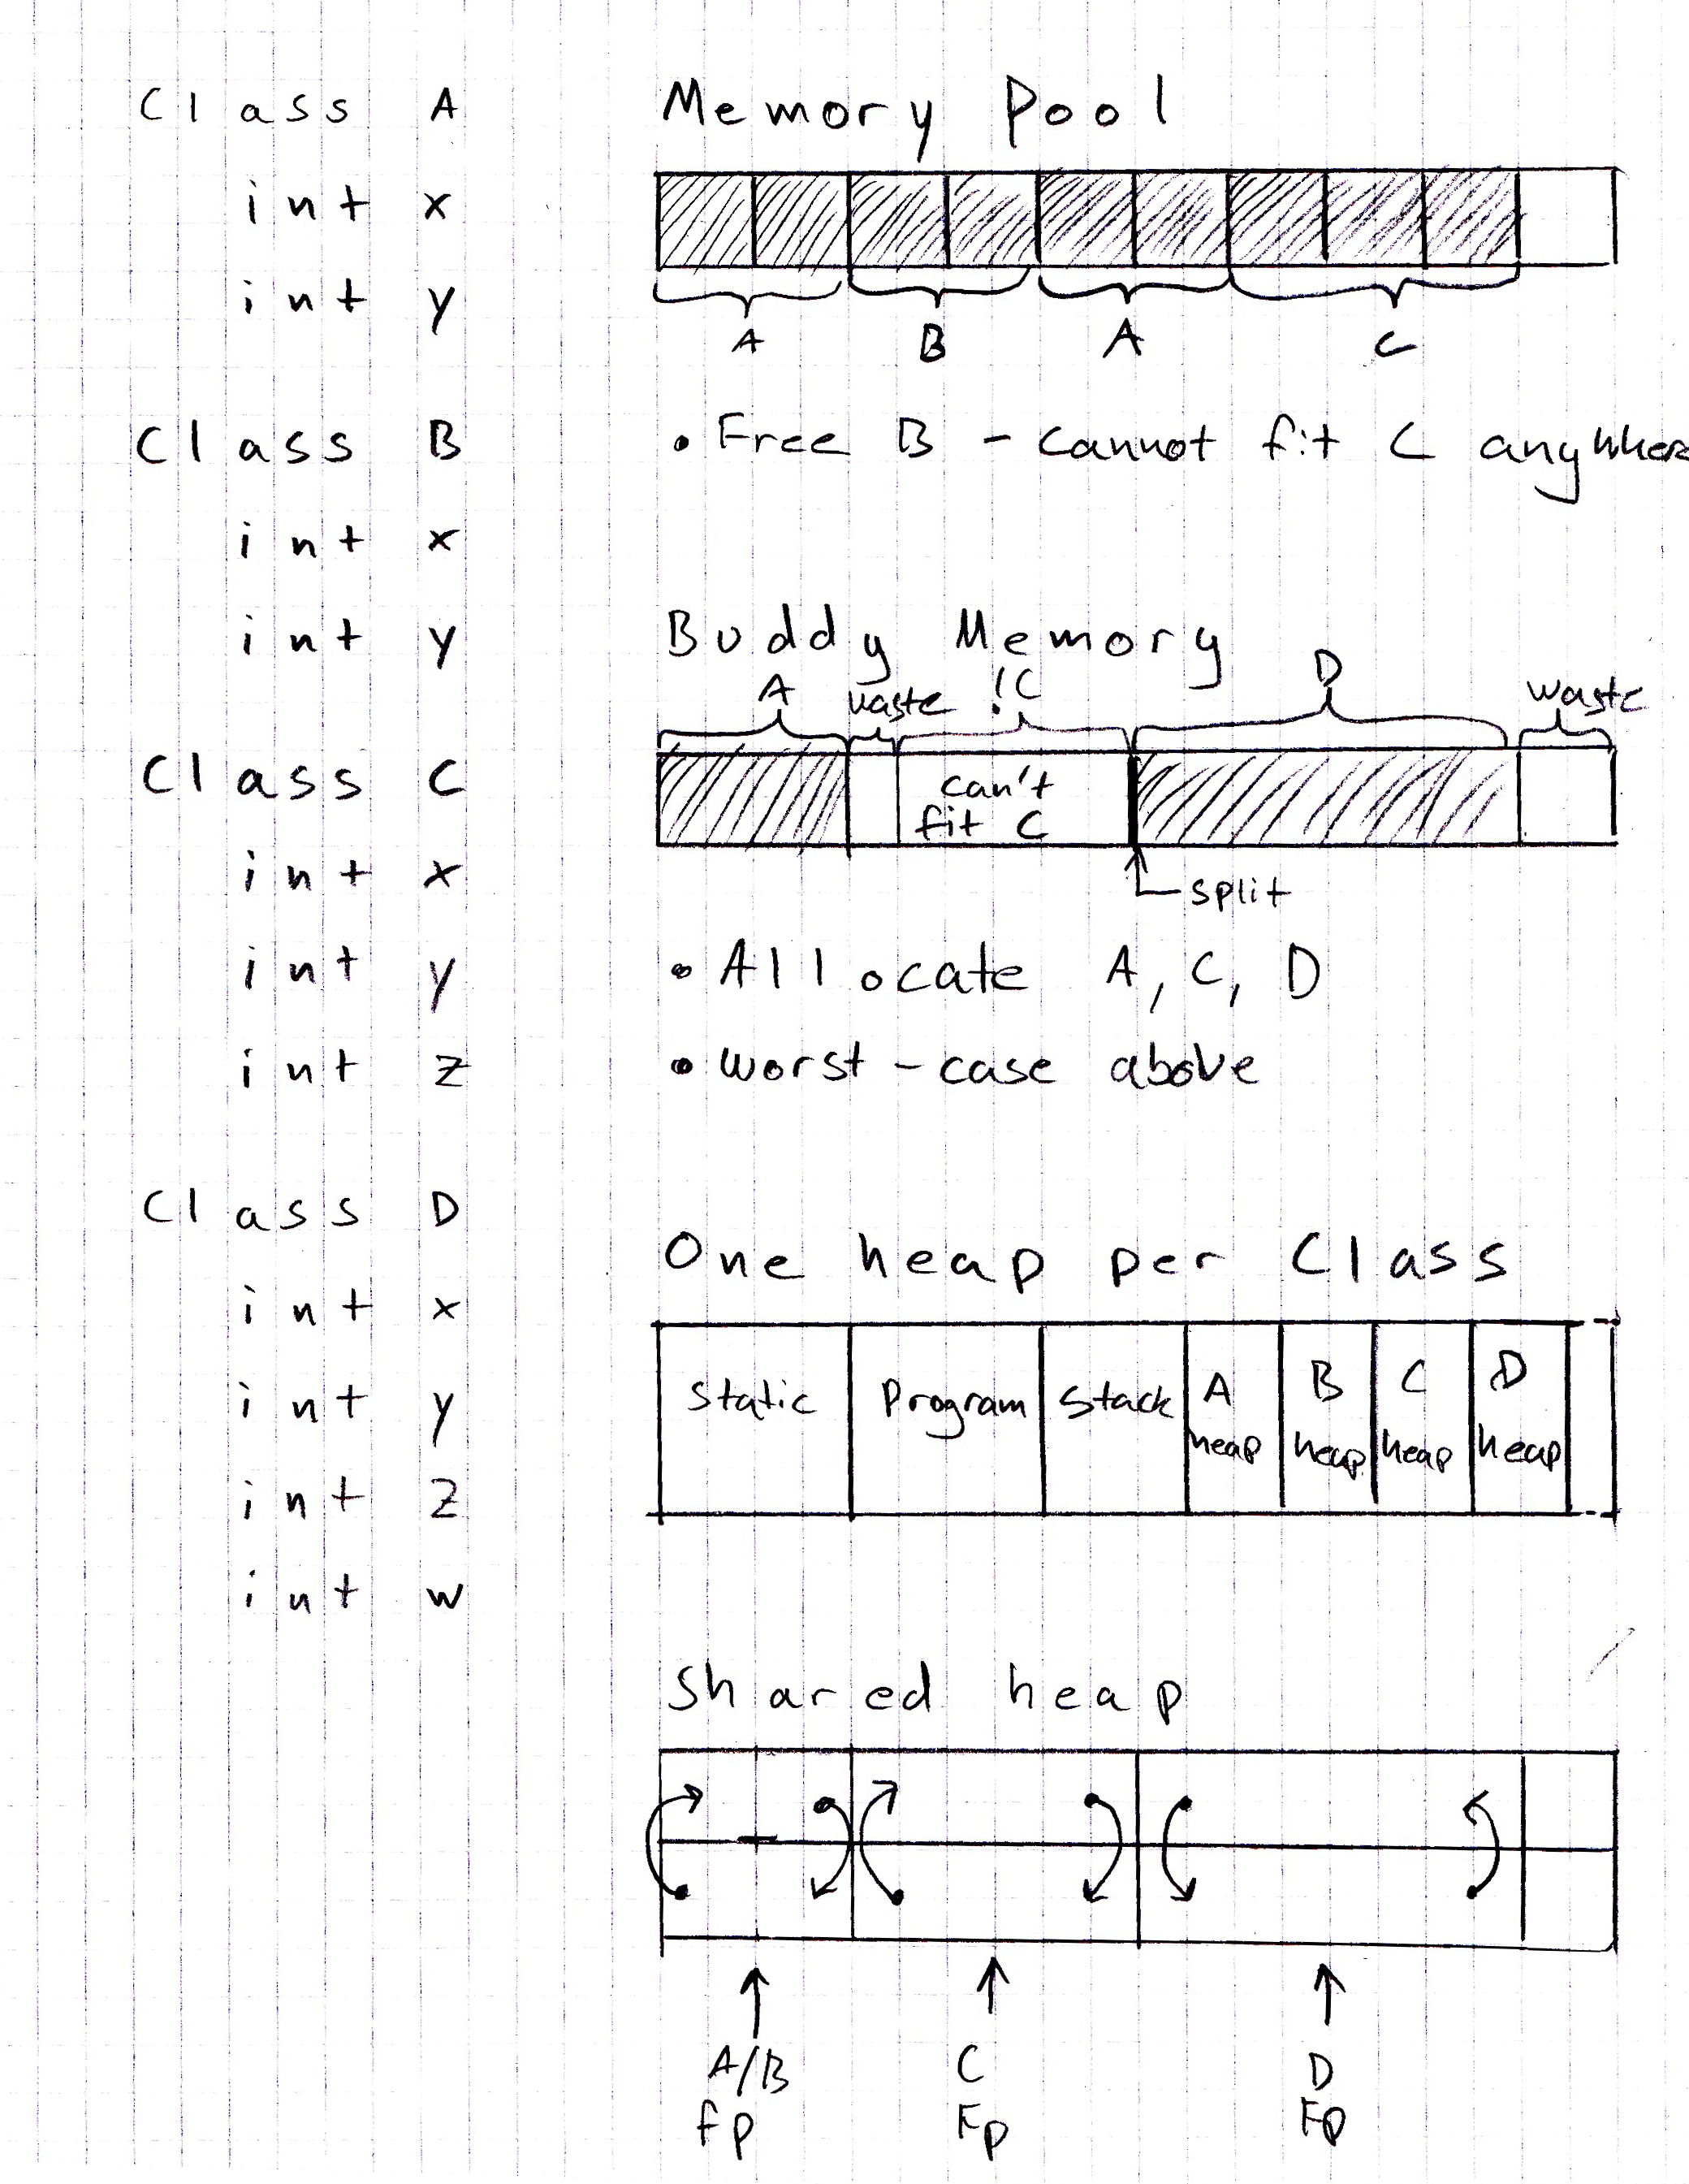
\includegraphics[width=0.7\textwidth]{heap-designs}
  \caption{Heap memory layouts (Draft)}
\end{figure}
